\documentclass[15pt,twosides,onecolumn,openany]{book}
\usepackage{graphicx} 
\usepackage[catalan]{babel}
\usepackage{emptypage}
\usepackage{hyperref}
\usepackage{mathtools}
\usepackage{blindtext}
\usepackage[utf8]{inputenc}
\usepackage{caption}
\usepackage{subcaption}
\usepackage{wrapfig}
\usepackage[a4paper]{geometry}
\geometry{top=2.5cm, bottom=2.5cm, left=2.5cm, right=2.5cm}
\usepackage{fancyhdr}
\pagestyle{fancy}
\usepackage{amsmath}
\usepackage{amssymb}
\usepackage{amsfonts}
\providecommand{\norm}[1]{\lVert#1\rVert}
\hypersetup{colorlinks=true,urlcolor=blue,linkcolor=blue}
\usepackage{multirow}
\usepackage{multicol}
\usepackage{rotating}
\usepackage{titlesec}

\newenvironment{Figura}
  {\par\medskip\noindent\minipage{\linewidth}}
  {\endminipage\par\medskip}

\titleformat{\section}  % comando de sección a formatear
  {\fontsize{14}{16}\bfseries} % formato para toda la línea
  {\thesection} % cómo mostrar el número
  {0.4em} % espacio entre el número y el texto
  {} 
  [] 

\fancyhf{}
\fancyhead[RO,LE]{\rightmark}
\fancyhead[LO,RE]{\leftmark}
\fancyfoot[RO,LE]{\thepage}
\fancyfoot[LO,RE]{Curs d'Introducció a LaTeX}

\renewcommand{\chaptermark}[1]{\markboth{\thechapter.\ #1}{}}
\renewcommand{\sectionmark}[1]{\markright{\thesection.\ #1}}

\graphicspath{ {images/} }

\begin{document}
\newpage
\thispagestyle{empty}
\begin{titlepage}
    \centering
    \vspace*{\fill}  
    {\Huge \textsc{Curs d'Introducció a \LaTeX{}} \par}
    \vspace{1cm}
    {\Large Optica't UAB \par}
    \vspace{0.5cm}
    {\large Versió 1.0 \par}
    \vspace{5cm}
    \vspace*{\fill} 
\end{titlepage}


\newpage

\thispagestyle{empty}
Benvolguts i benvolgudes a aquest text introductori de LaTeX. Som Optica't, un grup de divulgació d'òptica física format per estudiants de la Universitat Autònoma de Barcelona. Aquest text està pensat per a facilitar l'aprenentatge d'aquesta eina a alumnes que comencin els seus estudis universitaris. Clarament, està orientat a graus científics, el nostre aprenentatge de LaTeX es basa en les necessitats i la curiositat que hem desenvolupat al llarg dels cursos en carreres com física o nanociències. Tot i això, pensem que LaTeX és una eina molt útil per a més disciplines i esperem que molta gent pugui fer profit d'aquest curs.

\newpage
\tableofcontents
\pagestyle{empty}
\newpage
Agraïments
\newpage
\pagestyle{fancy}
\chapter{Introducció}
\thispagestyle{empty}

Dediquem aquest capítol a explicar des de zero com funciona LaTeX i com podem començar a crear els nostres primers documents. La finalitat del capítol és que us quedeu amb els conceptes bàsics de com funciona l'eina, la seva sintaxi, els possibles errors que trobareu, etc.

\section{Què és LaTeX i la seva utilitat}
LaTeX és un editor de textos que funciona de forma similar a un llenguatge de programació compilat. Està basat en el llenguatge de baix nivell \TeX{}, i està pensat principalment per a escriure textos científics de forma senzilla i elegant. La filosofia d'aquesta eina és que qui redacti no es preocupi del format del document, només en què ha d'escriure. A diferència d'un editor de textos \textsc{WYSIWYG} (en anglès, 'el que veus és el que obtens') al treballar amb LaTeX no podem veure el resultat del que redactem al moment d'escriure-ho. En LaTeX es treballa directament amb codi i després un compilador ho interpreta i genera un resultat (per exemple imprimeix el document per pantalla o genera un arxiu \texttt{.pdf}).\\\\
En un principi pot semblar que escriure en codi i no veure què és el que estem generant és contraproduent i pot fer menys atractiva la idea de treballar amb aquest editor i no amb altres més populars. Però, com veureu al llarg d'aquest text, aquest desavantatge queda opacat per la quantitat d'eines útils i de personalització que s'obtenen en treballar amb LaTeX.\\\\
Aquest curs se centra a abastar tot el necessari per a començar a escriure textos científics, com ara lliuraments de diverses assignatures de la carrera o per al treball de fi de grau. Però, en ser només un text introductori, no podrem explicar totes les eines que ofereix LaTeX bàsic i encara menys totes les eines que ha creat la comunitat. És necessari dir també que la utilitat d'aquest editor de textos va més enllà dels textos científics semblants a \textit{papers}. LaTeX té incorporades eines per a escriure llibres, per a escriure música, per a fer presentacions... Us convidem a informar-vos més enllà d'aquest text perquè podeu jugar amb totes les possibilitats que ofereix LaTeX tot i que no estudieu a cap branca científica.
\section{Entorns per a treballar amb LaTeX}
Per començar a treballar amb LaTeX primer necessitem saber on! És a dir, necessitem saber quin és el nostre entorn de treball. Igual que passa amb els llenguatges de programació, podem córrer LaTeX a dins d'una gran varietat d'entorns. Cada entorn és lleugerament diferent de l'altre, les seves característiques depenen de la versió i de quin sigui el flux de treball pensat específicament per a aquell entorn. Escollir un bon entorn pot arribar a ser una mica enrevessat, per tant, per a facilitar la tasca a les persones que encara no han fet servir LaTeX o que no estiguin familiaritzades en treballar amb programes de manera local centrarem el curs en l'entorn d'Overleaf. Sense ser exhaustius també parlarem sobre altres entorns com algunes eines d'escriptori o a escriure directament en un document de text amb eines més específiques de programació.\\\\
Per al lector o lectora que ja tingui experiència amb Overleaf i vulgui fer servir les altres eines, pròximament crearem una guia que complementi aquest curs amb més informació, de moment ens centrarem en que pugueu escriure el vostre primer document en LaTeX.
\subsection{Overleaf}
L'entorn per exce\lgem ència per a aprendre LaTeX i per a fer petits projectes co\lgem aboratius és Overleaf. Per a fer-ho servir no cal insta\lgem ar-se res, només necessites connexió a internet i un usuari. Overleaf és un entorn de LaTeX en línia pensat per a fer més fàcil la co\lgem aboració entre usuaris a l'hora de crear un document compartit. Els seus avantatges són:
\begin{itemize}
    \item No requereix cap insta\lgem ació, només tenir un compte. Per a poder accedir a un compte d'Overleaf només necessiteu un correu electrònic i entrar a la web oficial\footnote{Us deixem l'enllaç vigent actualment: \url{https://es.overleaf.com}}

    \item Interpreta el codi fins i tot si aquest conté algun petit error

    \item Permet treballar conjuntament amb diverses persones\footnote{Actualment (inici del 2025) la limitació per a editar el mateix projecte d'Overleaf es limita a dos usuaris. La resta d'usuaris que entrin al projecte només poden llegir-ho.}

    \item Permet classificar els teus projectes amb etiquetes

    \item Té insta\lgem ats alguns paquets que el LaTeX pur no té per defecte

    \item Té un sistema de navegació i una visualització del log de compilació intuïtius 

    \item Té integrades algunes eines que faciliten la generació de codi, com ara botons o \textit{short cuts} que canvien el format del text com en Word o un generador de taules buides

    \item Proporciona un editor visual on es pot treballar en un entorn semblant a un editor WYSIWYG
\end{itemize}
Com aquesta serà l'eina que farem servir a la resta del curs, explicarem una mica més sobre com funciona. Un cop tinguem obert un compte podrem crear un nou projecte des del menú principal. Overleaf ofereix moltes plantilles preestablertes, però per a aprendre treballarem amb una plantilla buida. Un cop obert el nou projecte en blanc veurem la següent pantalla:

\begin{figure}[h]
    \centering
    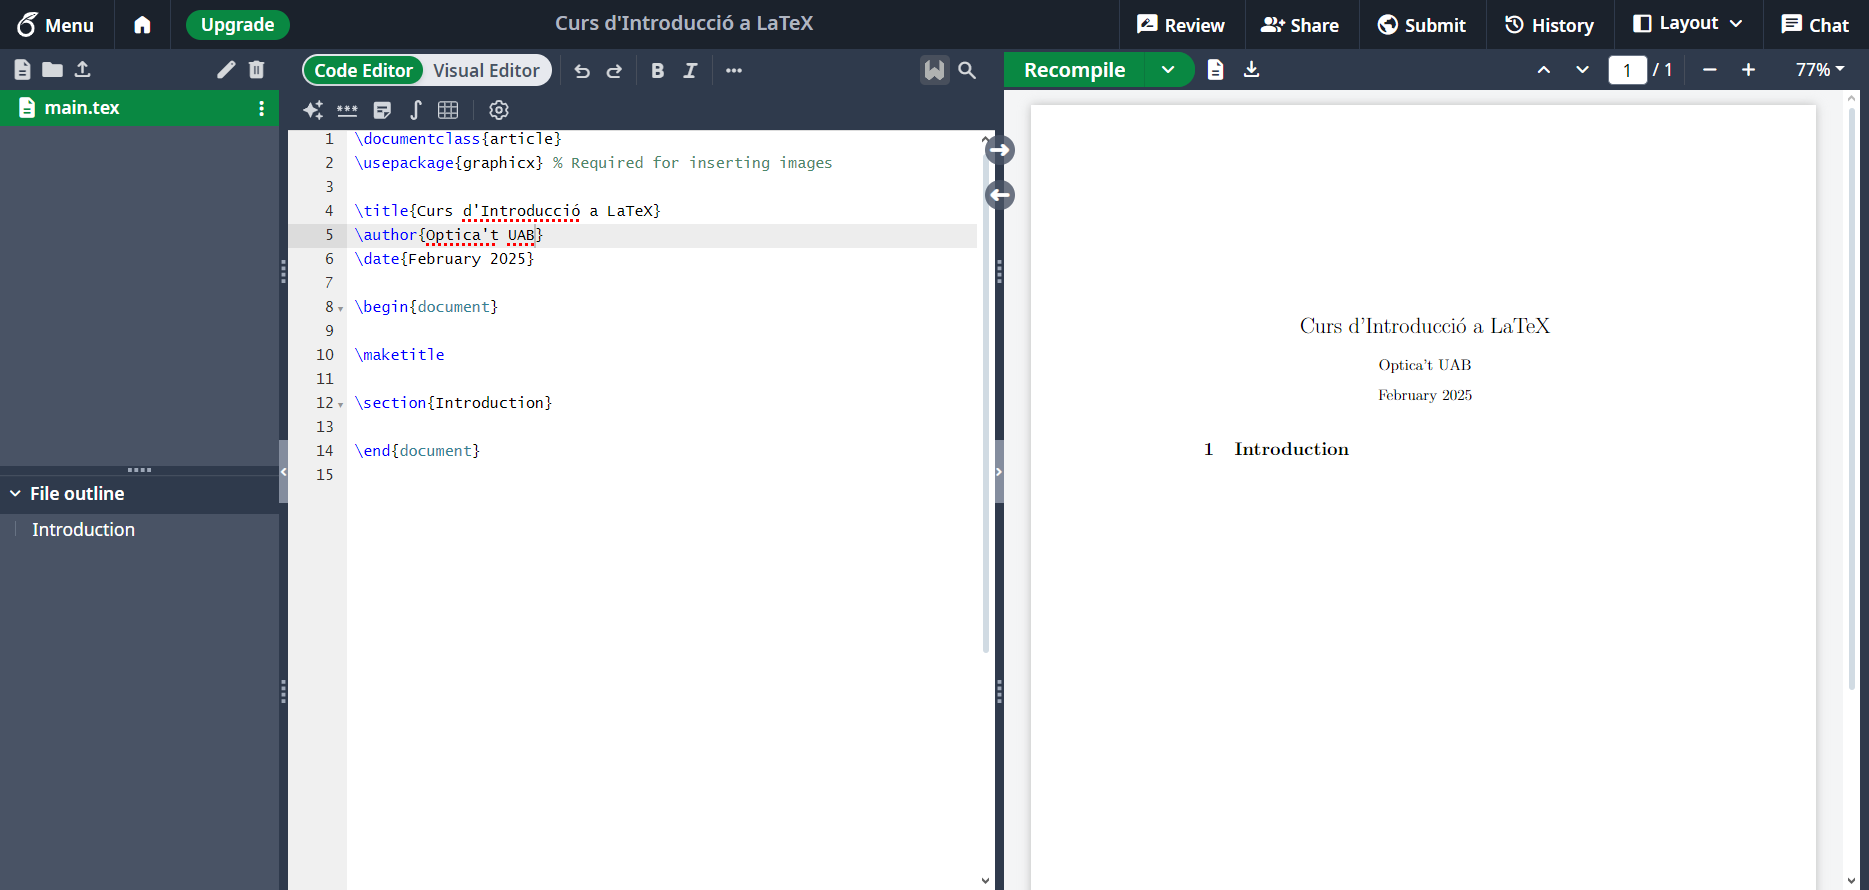
\includegraphics[width=0.95\linewidth]{../Text principal/Imatges/captura_nou_projecte.png}
    \caption{Entorn de treball d'Overleaf per a un projecte en blanc.}\label{fig:entorn_Ovlf_blanc}
\end{figure}

\noindent Observem de la Figura \ref{fig:entorn_Ovlf_blanc} que l'entorn se separa en tres parts. A l'esquerra del tot observem un menú, l'explorador d'arxius i de projecte. Aquest explorador funciona com a un gestor de carpetes i d'arxius, molt similar a l'explorador d'arxius de Windows. A la part superior de l'explorador aniran apareixent els arxius que fem servir al projecte. Podem mantenir un ordre d'aquests arxius utilitzant carpetes i canviant el nom de cada arxiu com vulguem. A la part inferior de l'explorador apareixerà un llistat de títols que ens serveixen per a moure'ns pel projecte de forma més senzilla, expliquem el seu funcionament amb més detall a la secció \ref{sec:cap_sec_subsec}.\\\\
A la dreta de la pantalla s'observa un visor pdf. Aquest visor permet veure per pantalla com va quedant el document que estem generant amb el codi que hem escrit. Notareu que a la part superior esquerra del visor hi ha un botó verd on posa \texttt{Recompile}. Cada cop que vulguem actualitzar el pdf amb la informació que hem escrit en codi hem de fer click a \texttt{Recompile}\footnote{No cal fer click sempre, existeixen dues alternatives. La primera és fer servir \textit{short cuts}, és a dir, prémer \texttt{Ctrl + s} o bé \texttt{Ctrl + Enter}. La segona és activar la funció automàtica de recompilat. Podeu accedir a aquesta opció desde el botó \texttt{Recompile}, prement la fletxa que té al costat.}. Diem a aquesta acció recompilar o compilar el codi.\\\\
Entre l'explorador i el visor tenim l'editor de text. Aquest editor és igual que qualsevol altre en programació. Allà és on escrivim totes les línies de codi necessàries per a generar el nostre document. Tot i això, aquesta finestra intermitja no sempre farà d'editor. Overleaf permet treballar amb més tipus d'arxiu que els de LateX com per exemple imatges. Per tant és més encertat pensar en l'editor com un entorn dinàmic de treball i no només com un simple editor de text.\\\\
Es pot configurar la visibilitat tant de l'editor com del visor pdf a partir de les opciones del desplegable \texttt{Layout}. Aquestes opcions deixen només visible un dels dos, els dos o permet separar-los en finestres diferents del navegador (això és útil si per exemple treballem a doble pantalla).
\subsection{LaTeX d'escriptori}
\subsection{Eines alternatives}
Per a la gent més experimentada o amb més interés en la programació deixem el següent entorn que, tot i potser semblar més complicat de fer servir, permet personalitzar completament el teu entorn de treball. LaTeX és un llenguatge, no un programa, per tant desde qualsevol editor de text podem escriure en LaTeX i, fent servir el compilador corresponent podrem generar la sortida que vulguem. Ara bé, existeixen eines que faciliten aquesta feina i ens permeten configurar el nostre entorn de forma més visual. Podriem fer una llista enorme amb eines de visualització útils i personalitzables, però una de les més populars (i des de la que s'està redactant aquest text) és Visual Studio Code. La instalació i configuració d'aquest entorn queda fora dels proposits d'aquest curs, però us convidem a informar-vos una mica sobre aquesta eina ja que no serveix només per a LaTeX. Visual Studio Code permet treballar amb LaTeX (i molts més llenguatges) en local, té integrat un explorador de directoris molt visual (no cal barallar-se amb la bash per a navegar per les carpetes) i permet afegir extensions pensades per a treballar amb LaTeX.
\section{Estructura bàsica d'un document}
\subsection{Sintaxi}
\subsection{Tipus de document}
\subsection{Paquets}
\subsection{Entorns}

\chapter{Format de text i estructura}
\thispagestyle{empty}
\section{Format del text pla}
\section{Justificació i espaiat del text}
\section{Llistes}
\section{Múltiples columnes}
\section{Estructura per a un document científic}
\subsection{Pàgina de títol i índex}
\subsection{Capítols, seccions i subseccions}\label{sec:cap_sec_subsec}
\subsection{Footnotes i etiquetes}
\subsection{Colorboxes}

\chapter{L'entorn matemàtic}
\section{Formes de cridar un entorn matemàtic}
\section{Sintaxi de l'entorn matemàtic}
\subsection{Operacions bàsiques}
\subsection{Parèntesis i claudàtors}
\subsection{Alguns accents, simbols i formats útils}
\subsection{Límits, sumatoris, productoris i integrals}
\section{Matrius i alineació}
\section{Exemples}

\chapter{Figures i taules}
\section{Figura}
\section{Subfigura}
\section{Taula}
\chapter{La bibliografia}
\section{L'arxiu \texttt{.bib}}
\section{Referenciar i imprimir la bibliografia}

\chapter{Personalització avançada}
\section{Paquets útils}
\subsection{babel}
\subsection{fancyhdr}
\subsection{hyperref}
\subsection{wrapfig}
\subsection{mhchem}
\end{document}